\documentclass[conference]{IEEEtran}
\IEEEoverridecommandlockouts
% The preceding line is only needed to identify funding in the first footnote. If that is unneeded, please comment it out.
\usepackage{cite}
\usepackage{amsmath,amssymb,amsfonts}
\usepackage{algorithmic}
\usepackage{graphicx}
\usepackage{textcomp}
\usepackage{xcolor}
\def\BibTeX{{\rm B\kern-.05em{\sc i\kern-.025em b}\kern-.08em
    T\kern-.1667em\lower.7ex\hbox{E}\kern-.125emX}}
\begin{document}

\title{An End-to-End solution to Autonomous Driving based on Xilinx FPGA}

\author{\IEEEauthorblockN{1\textsuperscript{st} Tianze Wu}
\IEEEauthorblockA{
\textit{Insititute Of Computing Technology Chinese Academy Of Sciences}\\
{University of Chinese Academy of Sciences}\\
Beijing, China \\
wutianze@ict.ac.cn}
\and
\IEEEauthorblockN{2\textsuperscript{nd} Weiyi Liu}
\IEEEauthorblockA{
\textit{Shanghai JiaoTong University}\\
Shanghai, China \\
liuweiyi@sjtu.edu.cn}
\and
\IEEEauthorblockN{3\textsuperscript{rd} Yongwei Jin}
\IEEEauthorblockA{
\textit{Xidian University}\\
Xian, China \\
yongweijin@outlook.com}
}

\maketitle

\begin{abstract}
Nowadays, the autonomous driving topic is very hot, many people are trying to provide a solution to this problem. This time we build our own auto-driving car based on Xilinx Pynq-Z2, it provides an end-to-end solution which inputs images from camera and outputs control instructions directly. The platform also uses the power of Deep learning Processing Unit(DPU) to accelerate the inference process and provides a simulator for training and testing in virtual environment. If the car meets some situations which cannot be handled by AI model, it's easy to add extra traditional computer vision functions to our control system. So our platform can help people who want to try autonomous driving build their own model and test it efficiently. We hope that our platform can be easy to use and extend.
\end{abstract}

\begin{IEEEkeywords}
Autonomous Driving, Machine Learning, Pynq-Z2, Field programmable gate arrays, Deep Learning Processing Unit
\end{IEEEkeywords}

\section{Introduction}
Autonomous Driving is getting more and more attention recently. The main problem to be solved in this area is how to meet the need of real-time computing. 
Though we now have many customized chips like GPU\cite{b1} and TPU\cite{b2} for machine learning acceleration, they are not able to provide both high performance and low power consumption. Also they are not flexible enough to adapt to different scenes. 

To meet these requests, FPGA\cite{b3} is a good solution since it can provide high performance and low power consumption, most important, people can build accelerators for specified algorithms easily.

This time we build our own auto-driving car based on Xilinx Pynq-Z2\cite{b4}, it provides an end-to-end solution to autonomous driving and it uses the power of DPU\cite{b5} to accelerate the computing. Our goal is to build a general and easy-to-use platform for those who want to try their own ideas about auto-driving.

We find that in previous FPT competitions\cite{b6}, many competitors use traditional computer vision methods or machine learning methods to detect objects and then make decisions based on the results\cite{b7}\cite{b8}. Our solution is quite different from theirs since we use a simple CNN model as our AI network and feed the model with pictures taken by the camera in the car and the model returns the control orders.
The platform we use is Xilinx’s Pynq-Z2 board, there is a DPU IP in its FPGA, with DPU’s help, we can accelerate the inference process of the model and make it possible to run AI inference task in limited resource platform like Pynq-Z2. 

We also build a simulator based on sdsandbox\cite{b9} using Unity3d\cite{b10}, we can collect training data, test the model's performance and pre-train the model in the simulator. It highly increases the efficiency and accelerates the project development. 

The rest of this paper is organized as follows. Section II describes the overview of our hardware structure and development environment. Section III presents the software architecture and details of methods we are going to use for the competition. Finally, the paper mentions the current progress and makes an conclusion.

\section{Overview of our car}

\subsection{Hardware structure}

The Fig.~\ref{co} is our robot car's photograph. Its body is made of acrylic board. There is one Pynq-Z2 board as the controller, it has a DPU IP for acceleration, the sensors we use now contains a camera only. The car has one capstan motor and one electric steering engine. Two rear wheels provide power while two front wheels provide steering capacity. We use two batteries to provide power, one for the Pynq board and one for the motors.

\begin{figure}[htbp]
\centerline{\includegraphics[width=0.5\textwidth]{car.jpg}}
\caption{Car overview.}
\label{co}
\end{figure}

\subsection{Development environment}

The operating system we use in the car is created by PetaLinux\cite{b11}, it has opencv and dpu support. We control the motors by directly writing values to physical memory address of FPGA, the drivers are implemented in FPGA. Most of our AI inference computing tasks are run by DPU, the tasks which DPU doesn't support are run by arm core embedded in Pynq-Z2. The driving decisions are made by AI model while the central controller is run in arm core.  

We provide two language implementations for collect-data module, you can collect data for training in c++ or python environment. The c++ version is more commonly used while the python version has a good support in Pynq-Z2. The auto-run module is implemented in c++ since the DNNDK-v3.0\cite{b12} version has only APIs for c++ language.

\section{Software Implementation and algorithms}

In most tasks, our solution can completely rely on machine learning methods, such as left-side driving, obstacle avoidance and crossroad driving. When it comes to other scenes, we use traditional computer vision algorithms and state machine to help us finish the task. The car only uses a camera as the sensor now, we may add some more sensors if a camera is not enough.

\subsection{Software architecture}\label{AA}

In our design, we aim to make the platform be easy to use and expand. There are three main modules in our system.

\begin{itemize}
\item The first part is Data Collect module. It needs human to control the car to finish some driving tasks. The program will record the images taken and real-time commands during the process. These data will be used as training data.
\item The second part is PC Host module. Since our edge devices cannot provide huge compution power, we will use more powerful devices like normal computers to do the machine learning job. You can use any hardware you like to do the training and then use DNNDK provided by Xilinx to do some optimizations. DNNDK kit can do pruning, quantization, compilation and optimization to the trained model. After this step, we will have DPU kernels that can help us accelerate inference process in the car.
\item The third part is Autonomous Driving module, it acts like the first module but the human controller of the car is replaced by machine learning network.
\end{itemize}

Since these three parts are separated, so it's easy to modify one module without affecting others. It will be easy to build a different neural network or use different hardware devices. We are also working on an virtual simulator for our platform, once it is finished you can train or evaluate the model based on virtual environment. This can help people build or test their model structure efficiently.
\begin{figure}[htbp]
\centerline{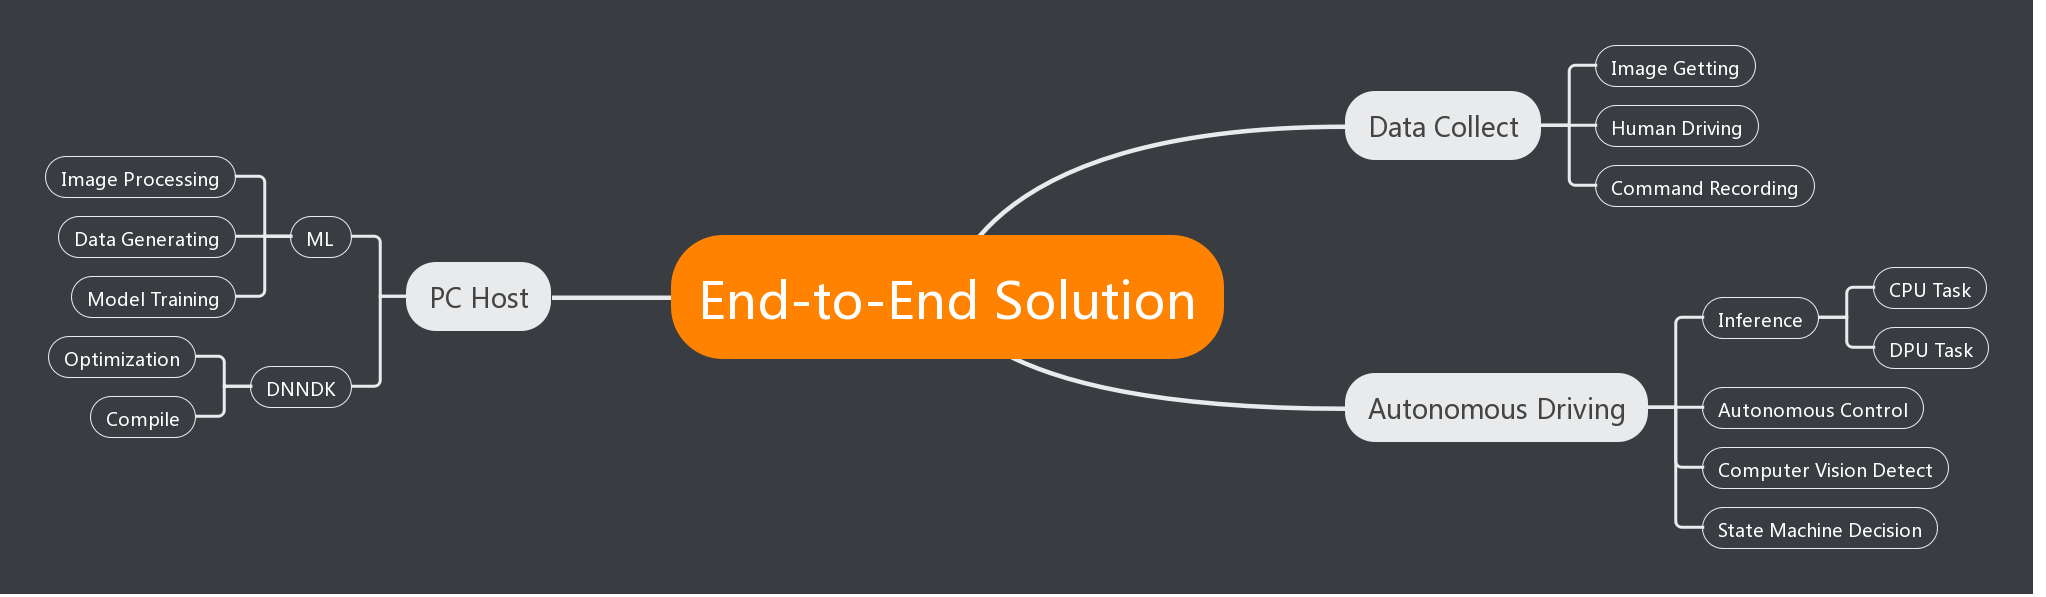
\includegraphics[width=0.5\textwidth]{software-architecture.jpg}}
\caption{Software Architecture}
\label{sa}
\end{figure}

\subsection{Work flow}

Fig.~\ref{wf} shows the control flow of our autonomous driving. The car can run in two mode, one is that the car will be in total control of machine learning methods, the other means that the traditional computer vision methods will be used when the car runs into the situation in which neural network is not able to handle.

The whole system will have one worker for running computer vision methods like objects recognition, one for taking photos and one for delivering instructions. The number of the workers for machine learning tasks can be specified since it's meaningful to run parallel tasks in DPU.

\begin{figure}[htbp]
\centerline{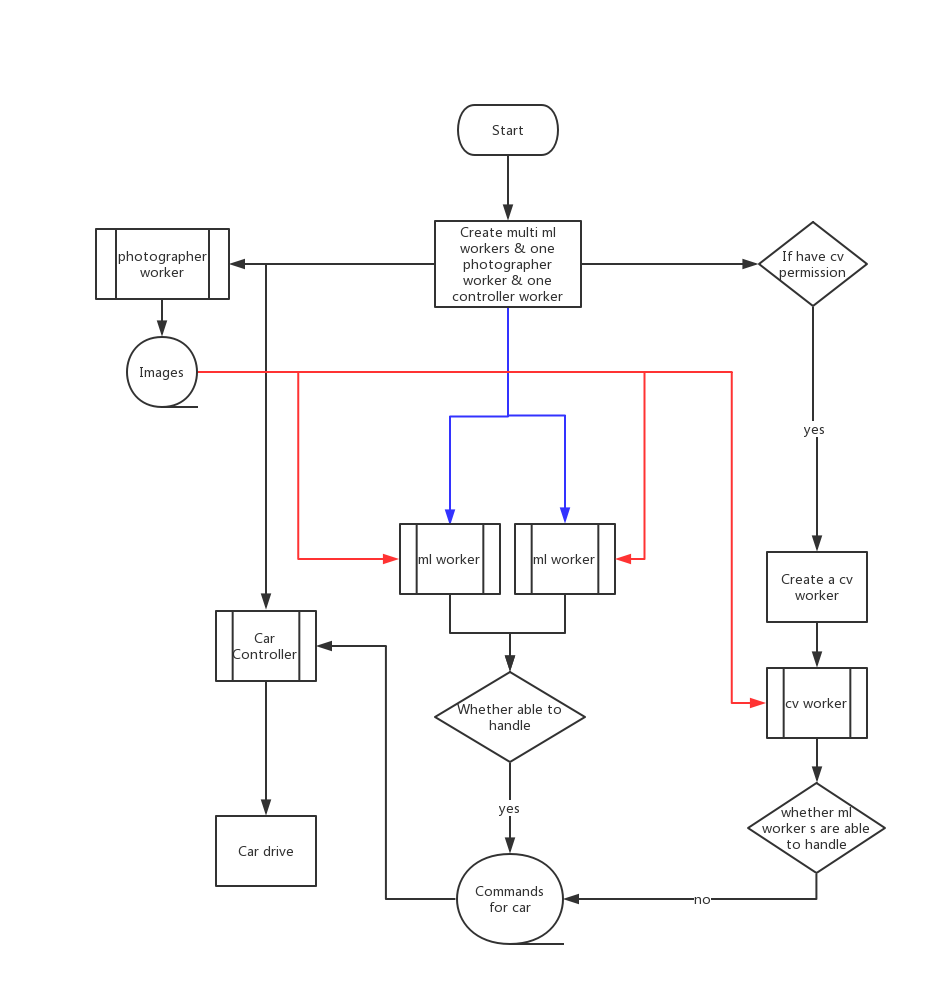
\includegraphics[width=0.5\textwidth]{workFlow.jpg}}
\caption{Work Flow}
\label{wf}
\end{figure}

\subsection{AI model}

The network we use is a simple end-to-end model. Since the DNNDK kit doesn't support some AI functions, we adapt our model to DNNDK. The structure of the model is shown in Fig.~\ref{ms}.  

\begin{figure}[htbp]
\centerline{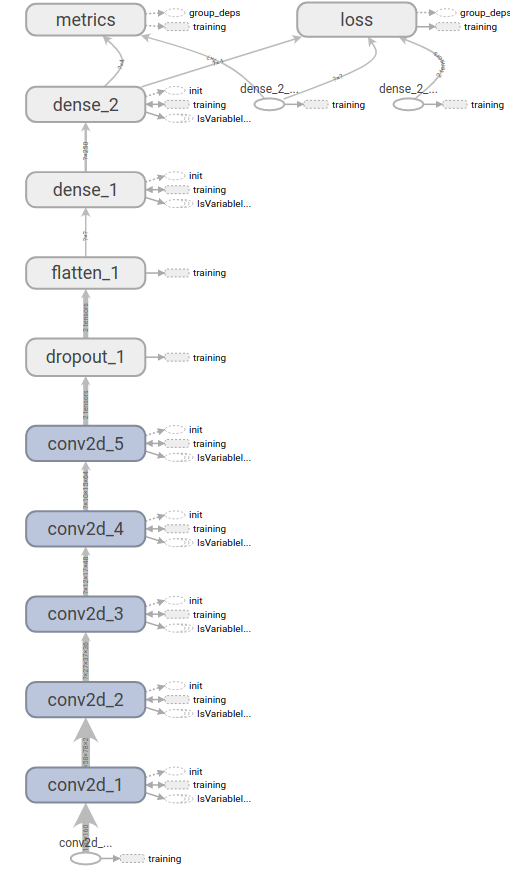
\includegraphics[width=0.5\textwidth,height=0.5\textheight]{net-structure.png}}
\caption{Model Structure.}
\label{ms}
\end{figure}

The main part of the model is CNN layers, they can extract features from the images taken by the car's front camera. Some fully connected layers follow the CNN layers, they can finally extract the command information needed for auto-driving. The activation function we use is Relu because it works well and can be accelerated by DPU. The last layer is a Softmax layer, it can provide classification and normalization functions for the model.  

Although the current model is not the perfect one and it cannot be accelerated by DPU totally, it's easy to make changes and optimizations to the model. With the development of DNNDK, more portion of the model can be accelerated and the whole system can be more efficient and powerful.

\subsection{Simulator}

Now we have built a simulator based on sdsandbox\cite{b9} to collect data for training, and we can also test our model using the simulator. With this tool, we can further separate software part from hardware part, even you don't have a real car, you can build and test your model in the virtual environment. The interface of our simulator is shown in Fig.~\ref{si}.  

\begin{figure}[htbp]
\centerline{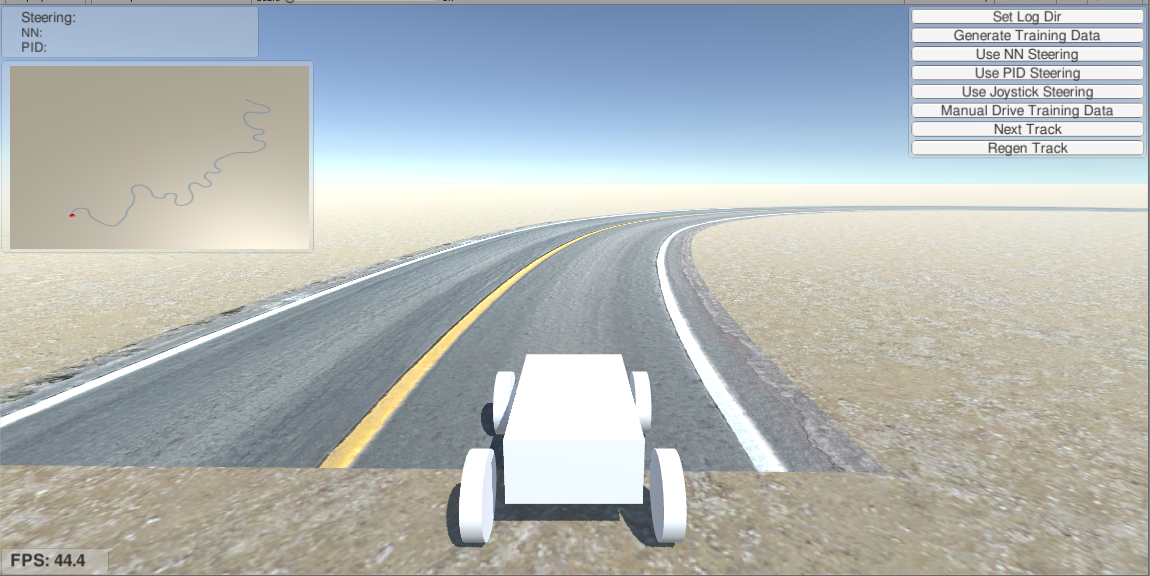
\includegraphics[width=0.5\textwidth]{simulator.png}}
\caption{Simulator Interface.}
\label{si}
\end{figure}

The main part of the model is CNN layers, they can extract features from the images taken by the car's front camera. Some fully connected layers follow the CNN layers, they can finally extract the command information needed for auto-driving. The activation function we use is Relu because it works well and can be accelerated by DPU. The last layer is a Softmax layer, it can provide classification and normalization functions for the model.  

Although the current model is not the perfect one and it cannot be accelerated by DPU totally, it's easy to make changes and optimizations to the model. With the development of DNNDK, more portion of the model can be accelerated and the whole system can be more efficient and powerful.

\subsection{Algorithms}
\begin{itemize}
\item Crossroad control. 

Since the AI model cannot handle the situation when the car meets a crossroad. We will help the car decide which direction to take according to the competition's request. The car will use neural network or cv algorithms to recognize all the scenes that need it to make a choice, for example the crossroad. After the car meets these scenes, first the main controller will tell the car which direction to take, then the car will use predefined control commands to drive through the crossroad. When this progress is finished, the AI model will retake the control of the car.
\item Image process. 

Although our solution is end-to-end, the training data needs to be processed. Now we just do the normalization to the input images, later we will try some more according to the evaluation of the model's performance.
\item Obstacle avoidance. 

For obstacle avoidance, traditional methods will first recognize the objects from the image and then use the state machine functions to make decisions. Our solution is quite different from it, we will add the obstacle avoidance scenes to the step of collecting training data. As a result, when the training step is finished, the AI model can avoid the obstacle automatically.
\item Road lane detection. 

To detect road lane, we first use 5*5 Gaussian filter to remove the noise of the image. Then Canny edge detection\cite{b13} is applied to detect the edges of the image. Hough transform\cite{b14} is employed to detect the lines of the image. Based on the orientation and relative position of detected lines, side line and stop line of the road can be identified. 

To improve the robustness and accuracy of the algorithm, more techniques will be added to the algorithm, such as K-Means clustering\cite{b15} for Hough lines, Kalman/Gabor filtering for sampled data, alternative IPM (inverse perspective mapping) lane detection method\cite{b16}.

Road lane detection algorithm is implemented in C++ with OpenCV. And it can be very time consuming running in ARM Cortex-A9 in Xilinx PYNQ-Z2. Some measures are taken to alleviate the heavy computational task of the algorithm. Firstly, the images captured by camera are cropped and down-sampled to reduce the computation complexity. Some time consuming tasks such as Gaussian filter, Canny edge detection, Hough transform are moved to FPGA using Xilinx xfopencv library\cite{b17}.

\item Traffic light recognition.

To recognize the traffic light in the contest, we first use IHLS color space\cite{b18} to remove the disturbance of the color in complicated background. After obtaining the color information, Hough circle transform\cite{b19} is applied to get the shape information of the traffic light. Combing the shape and color information, traffic light or similar objects can be detected. Finally, a simple BP neural network is employed to accurately recognize the traffic light in the contest.

Traffic light recognition algorithm is implemented in C++ with OpenCV. Similarly, it can be very time consuming running in ARM Cortex-A9 in Xilinx PYNQ-Z2. To reduce computation complexity, images captured by camera can be cropped as well since the traffic light only appear in the upper half of the image. Hough circle transform can be implemented in FPGA using Xilinx xfopencv library and BP neural network can be implemented in FPGA using Xilinx Vivado HLS.

\end{itemize}

\section{Development status}

Until now, we have built the whole system, the AI model works well in simple scenes in virtual environment. We are busy implementing the cv functions and optimizing the hardware structure of the car. Later we will try to make some improvements to the model and do some tests and modifications according to the competition's rules. 

\section{Conclusion}

The DPU embedded in FPGA accelerates the inference progress of AI algorithms. Our team wants to use this great power to build an autonomous driving system, with the help of Xilinx's Pynq-Z2 and DNNDK, our project will provide people with a new version of end-to-end autonomous driving solution.

We will focus on the stability of the system and the cooperations between AI network and traditional methods in the next step.

%\begin{table}[htbp]
%\caption{Table Type Styles}
%\begin{center}
%\begin{tabular}{|c|c|c|c|}
%\hline
%\textbf{Table}&\multicolumn{3}{|c|}{\textbf{Table Column Head}} \\
%\cline{2-4} 
%\textbf{Head} & \textbf{\textit{Table column subhead}}& \textbf{\textit{Subhead}}& \textbf{\textit{Subhead}} \\
%\hline
%copy& More table copy$^{\mathrm{a}}$& &  \\
%\hline
%\multicolumn{4}{l}{$^{\mathrm{a}}$Sample of a Table footnote.}
%\end{tabular}
%\label{tab1}
%\end{center}
%\end{table}

\section*{Acknowledgment}

The project is supported by Xilinx and Institute of Computing Technology Chinese Academy Of Science.

\begin{thebibliography}{00}

\bibitem{b1} Nurvitadhi, E., Sheffield, D., Sim, J., Mishra, A., Venkatesh, G., \& Marr, D. (2016, December). Accelerating binarized neural networks: Comparison of FPGA, CPU, GPU, and ASIC. In 2016 International Conference on Field-Programmable Technology (FPT) (pp. 77-84). IEEE.
\bibitem{b2} Jouppi, N. P., Young, C., Patil, N., Patterson, D., Agrawal, G., Bajwa, R., ... \& Boyle, R. (2017, June). In-datacenter performance analysis of a tensor processing unit. In 2017 ACM/IEEE 44th Annual International Symposium on Computer Architecture (ISCA) (pp. 1-12). IEEE.
\bibitem{b3} Mahajan, Divya, et al. "Tabla: A unified template-based framework for accelerating statistical machine learning." 2016 IEEE International Symposium on High Performance Computer Architecture (HPCA). IEEE, 2016.
\bibitem{b4} TUL PYNQ-Z2 [ONLINE] Available at: http://www.tul.com.tw/ProductsPYNQ-Z2.html  
\bibitem{b5} TUL DPU [ONLINE] Available at: https://www.xilinx.com/support/documentation/ ip\_documentation/dpu/v3\_0/pg338-dpu.pdf
\bibitem{b6} An FPGA design competition for developing autonomous driving robot cars is held in FPT2019 [ONLINE] Available at: http://fpt19.tju.edu.cn/Contest/FPT2019\_FPGA\_Design \_Competition/Contents\_and\_Conditions.htm
\bibitem{b7} Kojima, A., \& Nose, Y. (2018, December). Development of an Autonomous Driving Robot Car Using FPGA. In 2018 International Conference on Field-Programmable Technology (FPT) (pp. 411-414). IEEE.
\bibitem{b8} Aoto, M., Wada, Y., \& Numata, Y. (2018, December). Development of an FPGA Controlled" Mini-Car" Toward Autonomous Driving. In 2018 International Conference on Field-Programmable Technology (FPT) (pp. 400-402). IEEE.
\bibitem{b9} Tawn Kramer. (2019, September) sdsandbox [ONLINE] Available at: https://github.com/tawnkramer/sdsandbox
\bibitem{b10} TUL Unity3d Available at: https://unity.com/learn
\bibitem{b11} TUL PetaLinux [ONLINE] Available at: https://www.xilinx.com/support/documentation/sw\_manuals/xilinx2019 \_1/ug1144-petalinux-tools-reference-guide.pdf
\bibitem{b12} TUL DNNDK [ONLINE] Available at: https://www.xilinx.com/support/documentation/sw\_manuals/ai\_inference /v1\_5
\bibitem{b13} John Canny, "A Computational Approach to Edge Detection, "IEEE Transactions on Pattern Analysis and Machine Intelligence, pp.679-698, 1986.
\bibitem{b14} J. B. Burns, A. R. Hanson and E. M. Riseman, "Extracting Straight Lines," in IEEE Transactions on Pattern Analysis and Machine Intelligence, vol. PAMI-8, no. 4, pp. 425-455, July 1986.
\bibitem{b15} S. Selim, M. Ismail, "K-Means-Type Algorithms: A Generalized Convergence Theorem and Characterization of Local Optimality," Pattern Analysis and Machine Intelligence, IEEE Transactions on, vol. 6, no. 1, pp. 81-87, 1984. 
\bibitem{b16} Jun Wang, Tao Mei, Bin Kong and Hu Wei, "An approach of lane detection based on Inverse Perspective Mapping," 17th International IEEE Conference on Intelligent Transportation Systems (ITSC), Qingdao, 2014, pp. 35-38.
\bibitem{b17} Xilinx. (2019, Sep) Xilinx/xfopencv. [Online]. Available:  https://github.com/Xilinx/xfopencv
\bibitem{b18} Allan Hanbury and Jean Serra, "A 3d-polar coordinate colour representation well adapted to image analysis," in Proceedings of the Scandinavian Conference on Image Analysis (SCIA), 2003, pp. 804–811.
\bibitem{b19} M. Rizon et al., 2005, "Object Detection using Circular Hough Transform", American Journal of Applied Sciences 2, vol 12, pp. 1606-1609.
\end{thebibliography}
\vspace{12pt}

\end{document}
